%===================================== CHAP 2 =================================

\chapter{Background Theory}

\section{Artificial Neural Networks}

\textit{This was missing in the specialization project. Need to cover all concepts used later in the report. This includes all different layers of a neural network. The layers (dropout, pooling, etc) could perhaps be a separate section after this one.}

\subsection{The Neuron}

Artificial Neural Networks (ANNs) are inspired by the structure and behavior of a biological brain, but they are generally not intended to be realistic models. A neural network consist of interconnected nodes referred to as units. These correspond to a biological neuron, the basic computational unit of the brain, structured as illustrated in \textbf{Fig. \ref{fig1}}. The connections between the units in an  corresponds to a biological neuron's dendrites, which provide input signals, and its single axon, which produces output signals and is connected to other neurons. \\

\begin{figure}
    \begin{minipage}{0.5\textwidth}
        \centering
            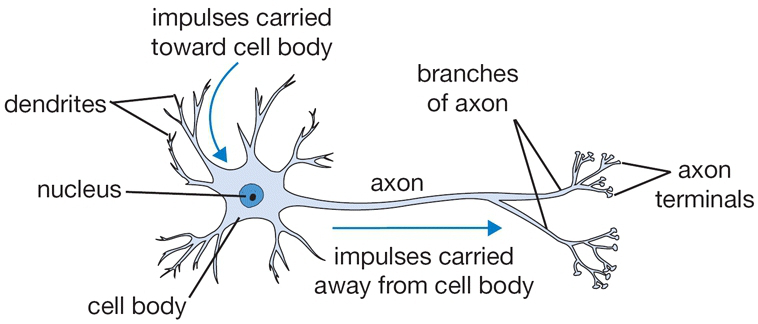
\includegraphics[width=1\textwidth]{fig/neuron}
            \caption{Biological neuron\cite{cs231n_part1}}
            \label{fig1}
    \end{minipage}
    \begin{minipage}{0.4\textwidth}
        \centering
            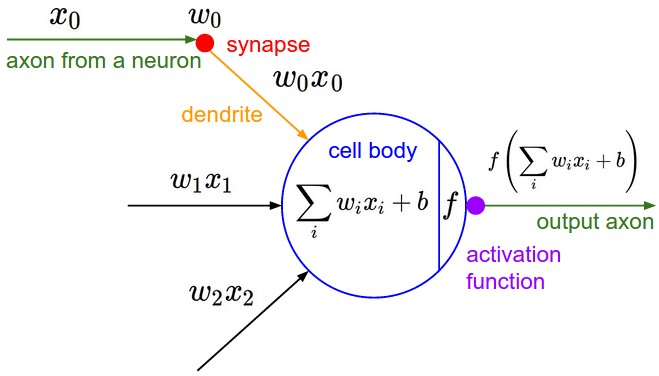
\includegraphics[width=1\textwidth]{fig/neuron_model}
            \caption{Mathematical model of a neuron\cite{cs231n_part1}}
            \label{fig2}
    \end{minipage}
\end{figure}

\noindent To simulate these signals, an ANN uses a mathematical model as illustrated in \textbf{Fig. \ref{fig2}}, where the signal is multiplied by the weight of a connection. The weight of a specific connection control how much the unit on one end influences the unit on the other end. The sum of all input signals are computed at the cell body of the unit. If this sum is above a certain threshold, the unit fires an output signal determined by its activation function by performing a specific mathematical operation on the sum.

\begin{itemize}
    \item The weights of a model can be learned by training the model on a set of input and output values.
\end{itemize}

\subsection{The Activation Function}

\noindent There are a great variety of activation functions in use, but we will only briefly describe those considered in our implementation. For further details we refer the reader to the Stanford CS class \textit{CS231n: Convolutional Neural Networks for Visual Recognition}\cite{cs231n_part1}.

\subsubsection{Sigmoid}

Describe the sigmoid function.

\subsubsection{Tanh}

Describe the tanh function.

\subsubsection{ReLU}

Describe the ReLU function.

\subsection{Architecture}

\begin{itemize}
    \item Input and output layers
    \item Fully-connected layer
    \item Hidden layers
    \item Deep models
    \item Convolutional layer
    \item Dropout layer
    \item Pooling
\end{itemize}

\section{Convolutional Networks}

\textit{More in-depth than covered in the specialization project. \\
What exactly is the convolutional operation? Convolutional layer (local connections and weight sharing) vs normal layer.}

\section{Residual Networks}

\section{Face Recognition}

\textit{Can probably use a lot from the specialization project here.}

\section{Facial Expression}

\textit{Here as well.}

\section{Visualization}

\textit{Describe all the different techniques, perhaps in more detail. \\
Possibly even implementation level.}

\cleardoublepage